% Copyright 2004 by Till Tantau <tantau@users.sourceforge.net>.
%
% In principle, this file can be redistributed and/or modified under
% the terms of the GNU Public License, version 2.
%
% However, this file is supposed to be a template to be modified
% for your own needs. For this reason, if you use this file as a
% template and not specifically distribute it as part of a another
% package/program, I grant the extra permission to freely copy and
% modify this file as you see fit and even to delete this copyright
% notice. 

\documentclass{beamer}

\usepackage[utf8]{inputenc}
\usepackage[T1]{fontenc}
\usepackage{graphicx}
\usepackage{amsmath,amssymb,amsfonts,textcomp}
\usepackage{url}
\usepackage{hyperref}

\usepackage{caption}
\usepackage{multirow}
% There are many different themes available for Beamer. A comprehensive
% list with examples is given here:
% http://deic.uab.es/~iblanes/beamer_gallery/index_by_theme.html
% You can uncomment the themes below if you would like to use a different
% one:
%\usetheme{AnnArbor}
%\usetheme{Antibes}
%\usetheme{Bergen}
%\usetheme{Berkeley}
%\usetheme{Berlin}
%\usetheme{Boadilla}
%\usetheme{boxes}
%\usetheme{CambridgeUS}
%\usetheme{Copenhagen}
%\usetheme{Darmstadt}
%\usetheme{default}
%\usetheme{Frankfurt}
%\usetheme{Goettingen}
%\usetheme{Hannover}
%\usetheme{Ilmenau}
%\usetheme{JuanLesPins}
%\usetheme{Luebeck}
\usetheme{Madrid}
%\usetheme{Malmoe}
%\usetheme{Marburg}
%\usetheme{Montpellier}
%\usetheme{PaloAlto}
%\usetheme{Pittsburgh}
%\usetheme{Rochester}
%\usetheme{Singapore}
%\usetheme{Szeged}
%\usetheme{Warsaw}

\title{End-to-end Sequence Labeling via Bi-directional
LSTM-CNNs-CRF}

% A subtitle is optional and this may be deleted
\subtitle{Paper Reimplementation}

\author{bacc. Bartol Freškura\inst{1} \and Assoc.~prof.~dr.~sc.~Jan Šnajder\inst{2}}
% - Give the names in the same order as the appear in the paper.
% - Use the \inst{?} command only if the authors have different
%   affiliation.

\institute[Faculty of Electrical Engineering and Computing] % (optional, but mostly needed)
{
  \inst{1}%
  Author\\
  Faculty of Electrical Engineering and Computing
  \and
  \inst{2}%
  Mentor\\
  Faculty of Electrical Engineering and Computing
}
% - Use the \inst command only if there are several affiliations.
% - Keep it simple, no one is interested in your street address.

\date{Masters Seminar, 2017}
% - Either use conference name or its abbreviation.
% - Not really informative to the audience, more for people (including
%   yourself) who are reading the slides online

%\subject{Theoretical Computer Science}
% This is only inserted into the PDF information catalog. Can be left
% out. 

% If you have a file called "university-logo-filename.xxx", where xxx
% is a graphic format that can be processed by latex or pdflatex,
% resp., then you can add a logo as follows:

% \pgfdeclareimage[height=0.5cm]{university-logo}{university-logo-filename}
% \logo{\pgfuseimage{university-logo}}

% Delete this, if you do not want the table of contents to pop up at
% the beginning of each subsection:

% Let's get started
\begin{document}

\begin{frame}
  \titlepage
\end{frame}

% Section and subsections will appear in the presentation overview
% and table of contents.

% You can reveal the parts of a slide one at a time
% with the \pause command:
\begin{frame}{Introduction}
  \begin{itemize}
  \item {
    Sequence labelling problems
  }
  \item {
      POS - \textit{Part of Speech} tagging and NER - \textit{Named Entity Recognition}
  }
  \item {
    Standard approach: graphical models like HMMs and CRFs
  }
  \item{
   New approach: deep neural architectures - RNNs and CNNs
  }
  \end{itemize}
\end{frame}


\begin{frame}{Paper Abstract}
    \begin{itemize}
    \item{
            Authors: Xuezhe Ma and Eduard Hovy from Carnegie Mellon University
            (2016)
        }
        \item{
            Sequence labelling via CNN-Bi-LSTM-CRF architecture
            }
        \item{
            State of the art results on the Penn Treebank WSJ and CoNLL 2003 datasets
            }
        \item{
            No task-specific resources, feature engineering, or data pre-processing is
            needed, except for word embeddings
        }
  \end{itemize}
\end{frame}


\begin{frame}{Architecture}
    \begin{itemize}
        \item{
            1-D Convolutional layer for character embeddings
            }
        \item{
            Pre-trained Glove word embeddings
            }
        \item{
            Bi-directional Long-short Term Memory (LSTM) for capturing word
            dependencies
            }
        \item{
            Conditional Random Fields layer for final sequence labelling
        }
  \end{itemize}
\end{frame}

\begin{frame}{Character embeddings layer}
    \begin{figure}
      \caption{Character embeddings layer followed by a 1-D convolutional layer.
      Max pool layer with stride=2 and size=2 is applied after the convolution.}
      \label{fig:cnn_embed}
      \centering
        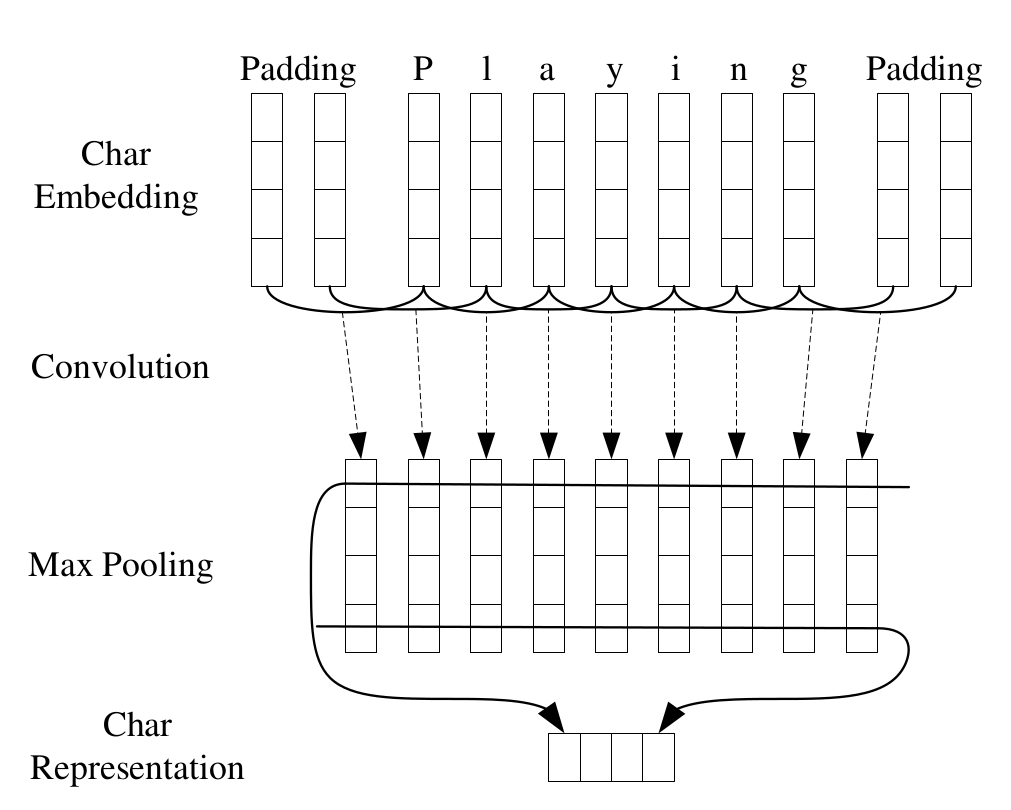
\includegraphics[width=0.5\textwidth]{imgs/cnn_embed.png}
    \end{figure}

\end{frame}

\begin{frame}{Pipeline}
    \begin{figure}
      \caption{Structure of the Bi-LSTM and CRF network layers.}
      \label{fig:pipeline}
      \centering
        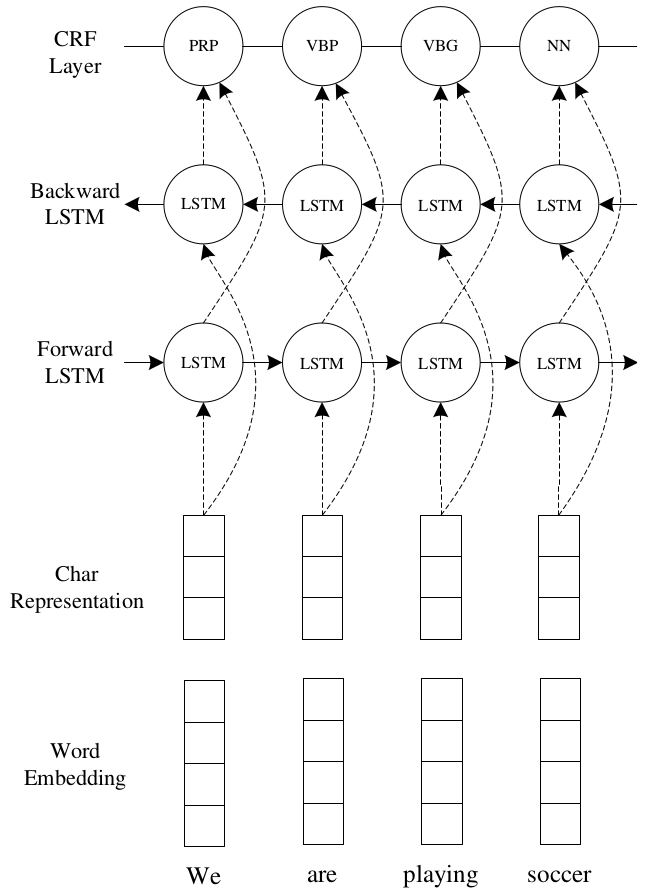
\includegraphics[width=0.35\textwidth]{imgs/pipeline.png}
    \end{figure}
\end{frame}

\begin{frame}{Parameters}
    \begin{itemize}
        \item{
            30 filters for the convolutional layer
            }
        \item{
             100-dimensional word embeddings
            }
        \item{
            Single layer Bi-LSTM with the hidden state size of 200
            }
        \item{
            Dropout layers with the dropout rate of 0.5
        }
        \item{
            Adam optimizer
        }
        \item{
            Early stopping for overfit prevention
        }
  \end{itemize}
\end{frame}

\begin{frame}{Datasets}
    \begin{itemize}
        \item{
            Sample of WSJ Treebank from the NLTK library
            }
        \item{
            45 unique POS tags
            }
        \item{
            Complete CoNLL 2003 dataset
            }
        \item{
            Categories: Persons, locations, organizations, and names of
            misc. entities
            }
        \item{
            Train set (60\%), Development set (20\%), Test set (20\%) with
            random shuffling
            }
    \end{itemize}
\end{frame}

\begin{frame}{Results}
    \begin{center}
        \begin{tabular}{ |c|c|c|c| }
        \hline
        &  & {\textbf{POS}} & {\textbf{NER}}\\ \hline
        \multirow{4}{*}{Development} & Accuracy & 96.73 & \textbf{98.80} \\
         & Precision & 93.77 & 93.73 \\
         & Recall & 93.91 & 94.02 \\
         & F1 & 93.52 & 93.56 \\ \hline
        \multirow{4}{*}{Test} & Accuracy & 96.71 & 98.23 \\
         & Precision & 93.73 & 91.45 \\
         & Recall & 93.80 & 91.90 \\
         & F1 & 93.45 & 91.30 \\ \hline
        \end{tabular}
        \captionof{table}{Results with dropout layers}
        \label{tab:dropout}
    \end{center}
\end{frame}

\begin{frame}{Results}
    \begin{center}
    \begin{tabular}{ |c|c|c|c| }
    \hline
    & & {\textbf{POS}} & {\textbf{NER}}\\ \hline
    \multirow{4}{*}{Development} & Accuracy & \textbf{97.08} & 98.78 \\
     & Precision & \textbf{94.24} & \textbf{93.69} \\
     & Recall & \textbf{94.28} & \textbf{94.13} \\
     & F1 & \textbf{93.97} & \textbf{93.63} \\ \hline
    \multirow{4}{*}{Test} & Accuracy & \textbf{96.98} & \textbf{98.32} \\
     & Precision & \textbf{94.14} & \textbf{91.73} \\
     & Recall & \textbf{94.19} & \textbf{92.22} \\
     & F1 & \textbf{93.87} & \textbf{91.63} \\ \hline
    \end{tabular}
    \captionof{table}{Results without dropout layers}
    \label{tab:no_dropout}
    \end{center}
\end{frame}



\begin{frame}{Results}
    \begin{center}
    \begin{tabular}{ |c|c|c|c| }
    \hline
    & & {\textbf{POS}} & {\textbf{NER}}\\ \hline
    \multirow{4}{*}{Development} & Accuracy & 77.63 & 51.89 \\
     & Precision & 84.80  & 63.25 \\
     & Recall & 83.89 & 53.90 \\
     & F1 & 82.42 & 49.09 \\ \hline
    \multirow{4}{*}{Test} & Accuracy & 78.16 & 48.32 \\
     & Precision & 84.68 & 61.47 \\
     & Recall & 83.95 & 50.84 \\
     & F1 & 82.65 & 46.12 \\ \hline
    \end{tabular}
    \captionof{table}{Results without the CRF layer}
    \label{tab:no_crf}
    \end{center}
\end{frame}

\begin{frame}{Conclusion}
    \begin{itemize}
        \item{
                Near identical results with the full blown architecture
            }
        \item{
                Huge differences when the CRF layer is removed
            }
        \item{
                Approach which can be generalized to any sequence labelling
                taks in NLP
            }
        \item{
                Poor character embeddings layer description
            }
        \item{
                Inverse dropout effect
            }
        \item{
                Further work: fastText and learning seperate character
                embeddings
            }
    \end{itemize}
\end{frame}

\begin{frame}{Q\&A}
    \begin{center}
    \Huge Questions?
    \end{center}
\end{frame}



\end{document}


